%%%%%%%%%%%%%%%%%%%%%%%%%%%%%%%%%%%%%%%%%%%%%%%%%%%%%%%%%%%%%%%%%%%%%%%%%%%%%%%%
%2345678901234567890123456789012345678901234567890123456789012345678901234567890
%        1         2         3         4         5         6         7         8

% \documentclass[letterpaper, 10 pt, conference]{ieeeconf}  % Comment this line out
                                                          % if you need a4paper
\documentclass[a4paper, 10pt, conference]{ieeeconf}      % Use this line for a4
                                                          % paper

\IEEEoverridecommandlockouts                              % This command is only
                                                          % needed if you want to
                                                          % use the \thanks command
\overrideIEEEmargins

\usepackage[pdftex]{graphicx} % modern graphics package
\usepackage[utf8]{inputenc}
\usepackage{amsmath} % assumes amsmath package installed
\usepackage{amssymb}  % assumes amsmath package installed
\usepackage{units}      % pretty units : \unit[val]{dim}
\usepackage{url}        % pretty urls
\usepackage{multirow}   % multiple rows in tables
\usepackage{fullpage}
\usepackage{siunitx}

\usepackage{times}


% Header and footer definitions
\usepackage{fancyhdr}
\renewcommand{\headrulewidth}{0.0pt}
\renewcommand{\footrulewidth}{0.5pt}

\pagestyle{fancyplain}
\fancyhf{}
\rfoot{\fancyplain{}{\thepage}}
\lfoot{\fancyplain{}{\today}}
\footskip = 30pt
\oddsidemargin = 15pt


\pagestyle{fancy}
\fancyhf{}
\rfoot[\today]{\thepage}
\lfoot[\thepage]{\today}
\cfoot[]{}



\graphicspath{{.}{./singlets/}{./search/}{./analysis/}{./CPG/}{./OpenQuestion/}}

\DeclareMathOperator{\sign}{sign}

\title{\LARGE \bf
Neural Networks miniproject - Single neuron model
}

\author{Douglas Watson and Dupont Thibault}


\begin{document}

\newcommand{\order}[1]{$\cdot 10^{#1}$}
\newcommand{\pvalue}[2]{p-value $< #1 \cdot 10^{#2}$}
\renewcommand{\thefigure}{\arabic{figure}}

\maketitle
\thispagestyle{fancyplain}



%%%%%%%%%%%%%%%%%%%%%%%%%%%%%%%%%%%%%%%%%%%%%%%%%%%%%%%%%%%%%%%%%%%%%%%%%%%%%%%%

\setcounter{tocdepth}{10}
\tableofcontents

\section{Introduction}
The purpose of the project is to study the role of dendrites in neural computation. To reach this goal, we first explore the effect of activation of different type of somatic ion channels on the somatic potential, using computer simulations based on the Hodgkin-Huxley model. In the second part we connect dendrites with different properties, each carrying either excitatory or inhibitory synapses, and we explore their respective contributions to the somatic potential. \\

\section{Hodgkin-Huxley model}




\subsection{Electrical model}



\subsubsection*{HH model}

In this project, the Hodgkin-Huxley (HH) model of neurons is used. The soma is represented as a capacitor, whose charge is affected by ion channels and an external stimulus. Each ion channel is described by a conductance and a reversal potential, and the external stimulus is modelled as a perfect current source. Fig. \ref{fig:HH_model} shows the electric model of a HH neuron. More information about this model can be found in the second lectures of prof. G. Wulfram in the courses titled “Neural Network and biological modeling” \cite{course}. \\

\begin{figure}
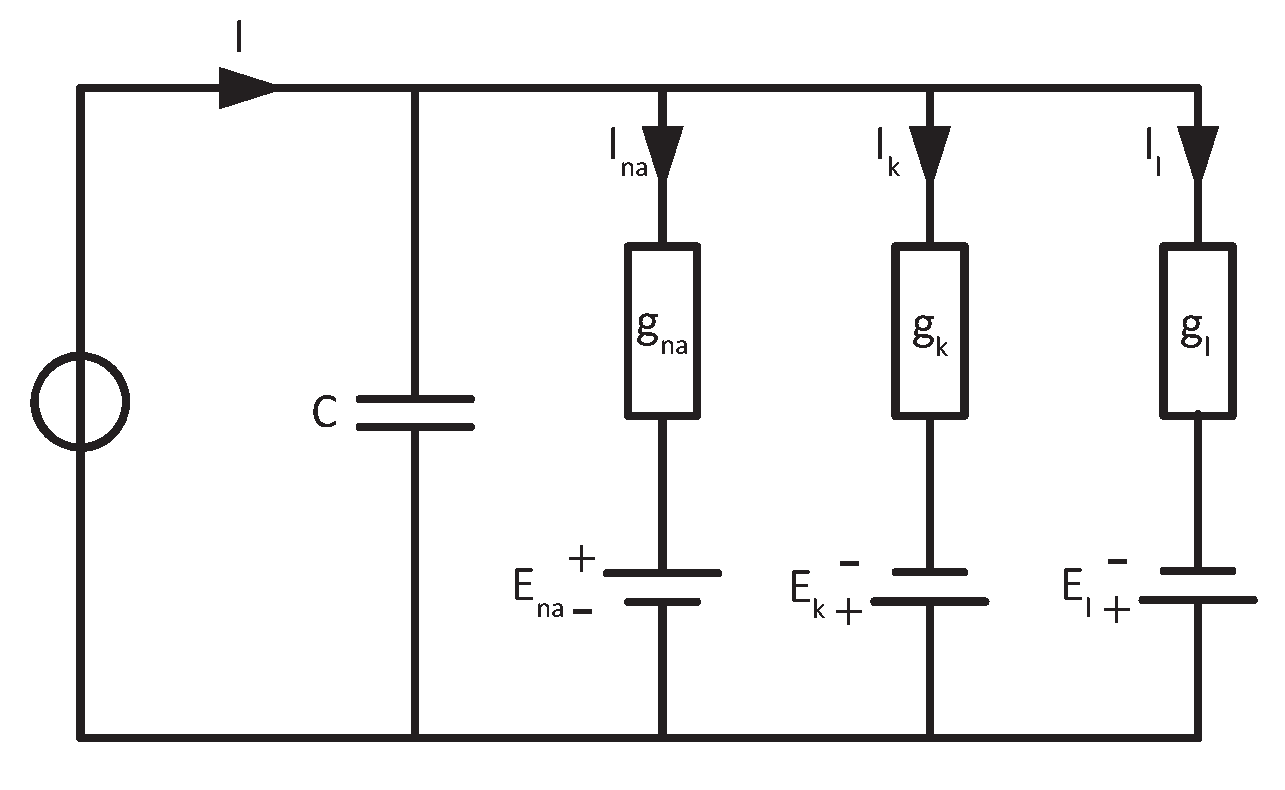
\includegraphics[width=\columnwidth]{figures/HH_model.pdf}
\label{fig:HH_model}
\caption{Hudgkin-Huxley electrical model}
\end{figure}






\subsubsection*{HH$_{x}$ and HH$_{xx}$ model}
For our project, we created two other models derived from the $HH$ model. We added another type of ion channel that provides a fourth source of current through the membrane. This current is called $I_{x}$ or $I_{xx}$ and transforms the model respectively to the $HH_{x}$ or $HH_{xx}$ models. Fig. \ref{fig:HHx_model} shows the $HH_{x/xx}$ electrical models.\\

\begin{figure}
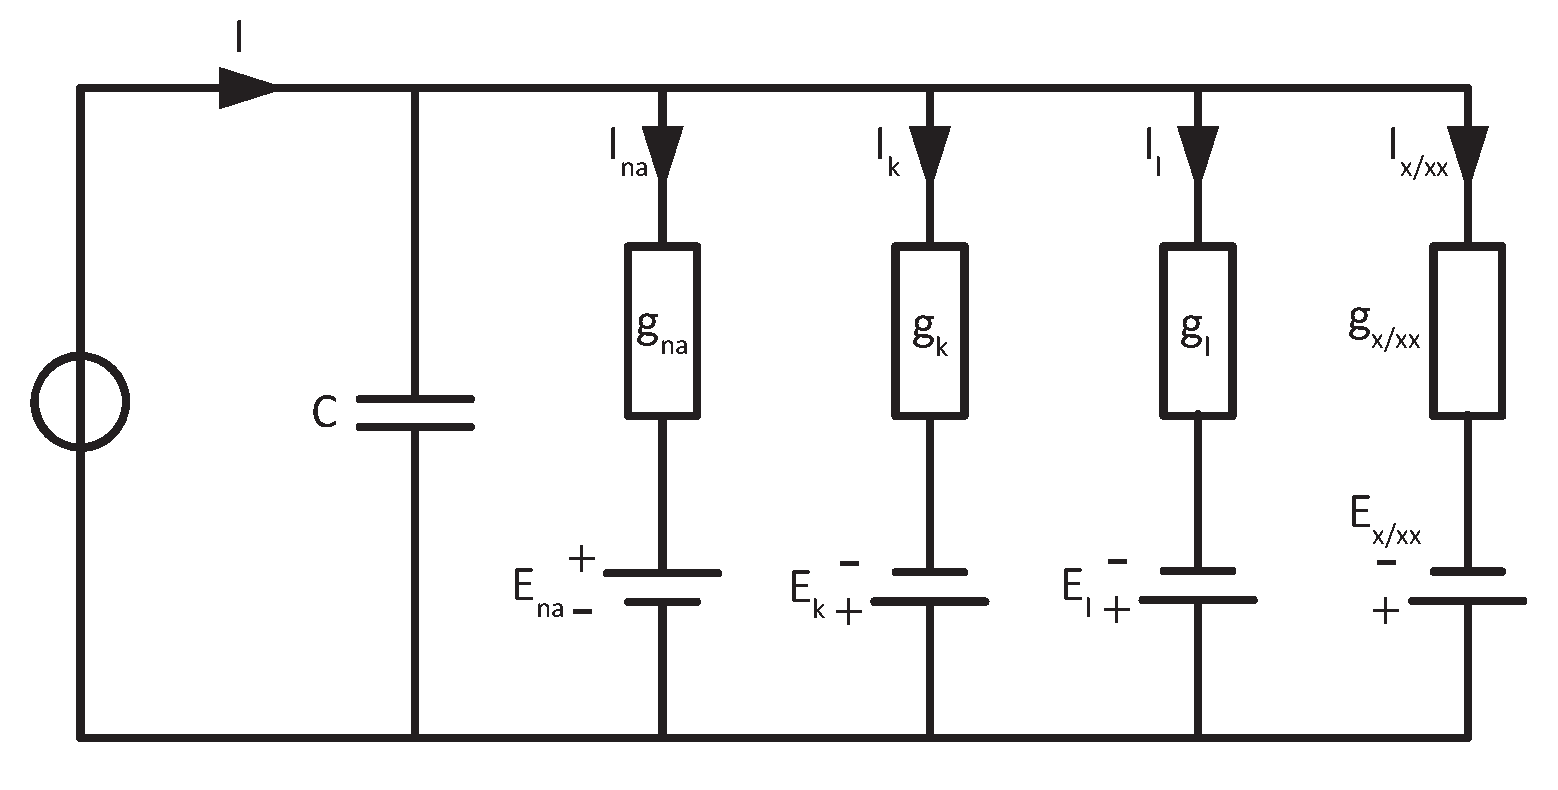
\includegraphics[width=\columnwidth]{figures/HHx_model.pdf}
\label{fig:HHx_model}
\caption{The $HH_{x/xx}$ models}
\end{figure}






\subsection{Mathematical model}
According to the Hodgkin-Huxley model, the net current flow through the membrane is the sum of the currents due to every kind of ion channel. For the standard $HH$ model the potential variation is describefd by :

\begin{equation}
\begin{split}
C \cdot \frac{du}{dt} =& I_{NA} - I_K - I_{Leak} + I(t) \\
= &-g_{NA} \cdot m(u)^3 \cdot h(u) \cdot (u-E_{NA})\\
&-g_K \cdot n(u)^4 \cdot (u-E_K)\\
&-g_L \cdot (u-E_L)\\
&+I(t)
\end{split}
\end{equation}

where, m(u), h(u) and n(u) are gating variables, that represent the opening of each channel. \\

To find the equation for the model $HH_{x/xx}$, we just add the $I_{x/xx}$ current to the $HH$ model : 

\begin{equation}
\begin{split}
C \cdot \frac{du}{dt} =& I_{NA} - I_K - I_{Leak} + I_{x/xx} + I(t) \\
= &-g_{NA} \cdot m(u)^3 \cdot h(u) \cdot (u-E_{NA})\\
&-g_K \cdot n(u)^4 \cdot (u-E_K)\\
&-g_L \cdot (u-E_L)\\
& - g_{x/xx} \cdot (u-E_{x/xx})^2\\
& +I(t)
\end{split}
\end{equation}

An important thing to notice is that I$_\text{x}$ and I$_\text{xx}$ depend of the tension difference squared. This implies that $I_{x}$ and $I_{xx}$ always flow in the same direction, independently of the membrane potential. This direction is determined by the sign of g$_\text{x/xx}$. If g$_\text{x/xx}<0$ the current push positive ion out of the cell, otherwise it transports the ions into the cell. In our case g$_\text{x}$ = \SI{5e-5}{\siemens} and g$_\text{xx}$ = \SI{-5e-6}{\siemens} \\





\subsection{Synapses}
The project involves a study on the influence of activated synapses on different parts of the neuron: the soma and the dendrites. We determine how sensitive the neuron is to external stimuli. Each synapse contributes an equal current through the membrane, which is equivalent to a single channel opening with a higher conductance. The total (summed) conductance for each types of synapse is therefore:

$$
g^{total}_{channel} = N \cdot g_{channel}
$$
with N = number of active synapses. In other words, the higher the number of activated synapses, the higher the total conductance of the channel.






\section{Model exploration}
In the first part, all models were parametrized with : soma$_\text{length}$ equal to \SI{67}{\micro\meter}, soma$_\text{diameter}$ equal to \SI{67}{\micro\meter}, inter-cellular resistivity equal to \SI{100}{\ohm\centi\meter}, membrane capacitance equal to \SI{1}{\micro\farad\per\centi\meter\square}, a passive mechanisms with g$_\text{pas}$ equal to \SI{0.15}{\milli\siemens\per\centi\meter\square}  and a reversal potential of \SI{-20}{\milli\volt}. The temperature is set to \SI{36}{\celsius}. The dendrites connected to the soma have : time constant = \SI{2}{\milli\second} and reversal potential = \SI{0}{\milli\volt}. \\

The difference between models comes from the maximum conductance and additional ion channel. g$_\text{HH,max}$ = \SI{0.005}{\micro\siemens}, g$_\text{HHx,max}$ = \SI{0.01}{\micro\siemens} and g$_\text{HHxx,max}$ = \SI{0.001}{\micro\siemens}. For the HH$_\text{x}$ and HH$_\text{xx}$ models we added respectively the I$_\text{x}$ and the I$_\text{xx}$ current. \\

All simulations were carried out using the Python interface to NEURON Release 7.1, and Python version 2.6.6 on Ubuntu Linux 10.10. \cite{website:neuron}\\







\subsection{Types I or II}
We first augment the stimulus current for each model and measured the spiking frequency to determine the type of each model.

Based on fig. \ref{fig:1_2}, all three models appear to be of Type I. But, to be sure of that, more points would be needed around the threshold current, to accurately determine whether the frequency increases smoothly from zero or makes a step.


\begin{figure}
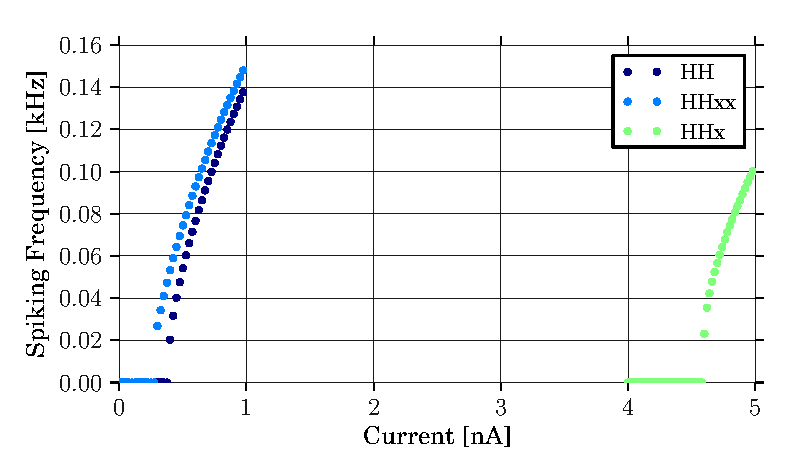
\includegraphics[width=\columnwidth]{../figures/1_2-neuron_type.pdf}
\label{fig:1_2}
\caption{The $HH_{x/xx}$ models}
\end{figure}







\subsection{Synapses opening and spikes}
To determine how many active synapses are needed to evoke a spike, we measure somatic potential with different numbers of active synapses, observing at what point a spike appears. \\

As we can see on figures \ref{fig:1_3a}, \ref{fig:1_3b} and \ref{fig:1_3c}, the models HH needs 5 active synapses to generate a spike, HH$_\text{x}$ need 24, and whereas of HH$_\text{xx}$ only needs 4 of them. We can also notice that the models HH and HH$_\text{xx}$ spike several times, whereas HH$_\text{x}$ stabilises itself after a single spike. To explain that, we should pay attention to the currents. \\

The value of g$_\text{x}$ explains both phenomena: g$_\text{x}$ = \num{5e-5} $>$ 0, this signifies that the I$_\text{x}$ current flows out of the membrane; in other words positive ions flow out. This fast depletion of ions from the soma inhibits spikes. Thus, to compensate for this large leak current, the soma needs much more ions to flow in, and therefore more open synapses. To spike several times, much more current would be needed --- values never reached with just 40 synapses. The negative sign of g$_\text{xx}$ indicates that it brings current in and therefore favours spiking, resulting in a lower synaptic threshold for HH$_\text{xx}$. \\

\begin{figure}
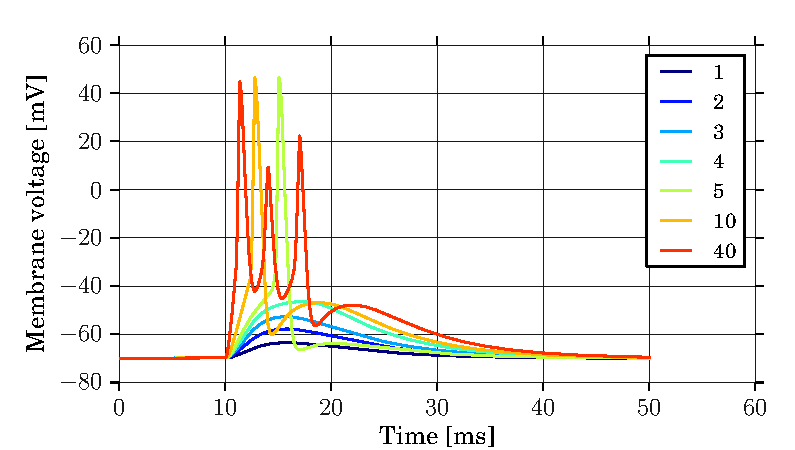
\includegraphics[width=\columnwidth]{../figures/1_3-HH_synapse_number.pdf}
\label{fig:1_3a}
\caption{HH model spike in function of the number of activated synapses}
\end{figure}

\begin{figure}
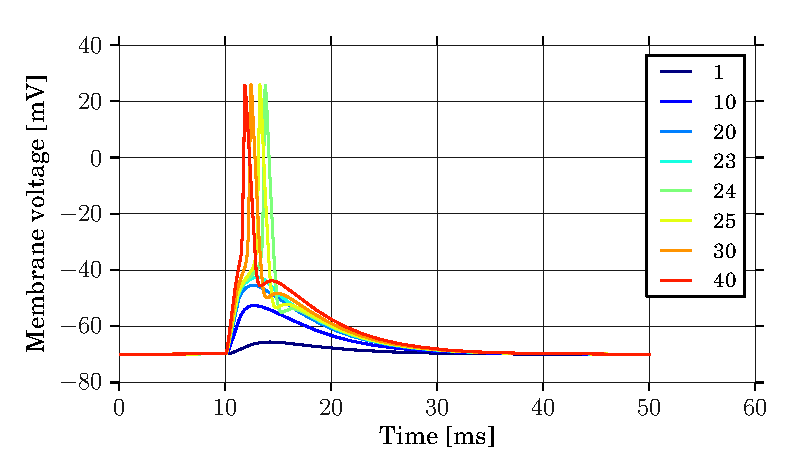
\includegraphics[width=\columnwidth]{../figures/1_3-HHx_synapse_number.pdf}
\label{fig:1_3b}
\caption{HH$_x$ model spike in function of the number of activated synapses}
\end{figure}

\begin{figure}
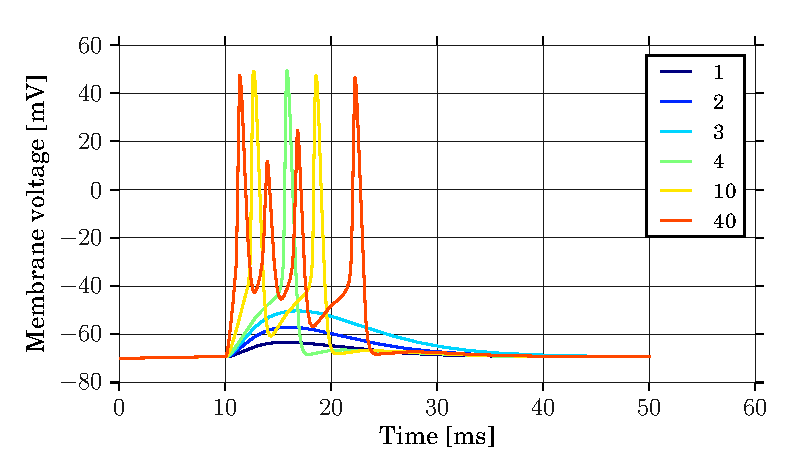
\includegraphics[width=\columnwidth]{../figures/1_3-HHxx_synapse_number.pdf}
\label{fig:1_3c}
\caption{HH$_{xx}$ model spike in function of the number of activated synapses}
\end{figure}






\subsection{Maximum somatic potential: synaptic integration}
Fig. \ref{fig:1_4} shows the amplitude of the somatic EPSP as a function of the number of active synapses. \\

\begin{figure}
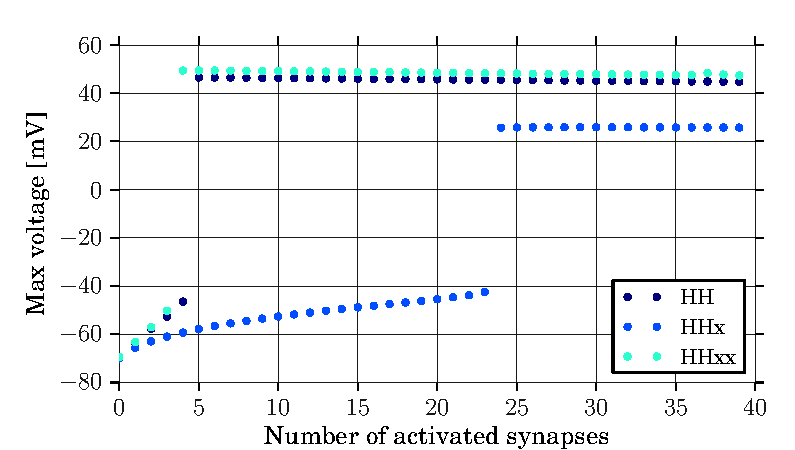
\includegraphics[width=\columnwidth]{../figures/1_4-number_of_synapses.pdf}
\label{fig:1_4}
\caption{Maximum somatic voltage in function of the number of activated synapses for each models}
\end{figure}


We notice the same spiking thresholds as previously, and we can now comment on the shape of the potential response in the subthreshold regime. HH$_\text{x}$ and HH$_\text{xx}$ show non-linear growth of the potential with regard to the number of activated synapses. This comes from the quadratic current dependence in HH$_\text{x}$ and HH$_\text{xx}$. The effect is more obvious for HH$_\text{x}$, because its conductance term is one order of magnitude larger than for HH$_\text{xx}$. \\





\subsection{Answer to 1.5}
The two channels differ by their conductance and by their reversal potential. In particular, the conductance of I$_\text{x}$ and I$_\text{xx}$ are respectively positive and negative. Therefore, in the subthreshold regime, I$_\text{x}$ tends to increase membrane potential (when it is away from the reversal potential), whereas I$_\text{xx}$ tends to decrease the potential. \\











\section{Space - time integration of dendrites}


\subsection{Setup}
The kind and the number of synapses on dendrites influences the behaviours of the soma. To prove it, we simulated the setup shown in fig. \ref{fig:soma_dendrites}, consisting of a soma and three dendrites.

\begin{figure}
\begin{center}
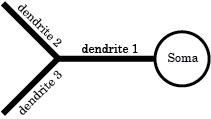
\includegraphics[width=4cm]{figures/soma.png}
\end{center}
\label{fig:soma_dendrites}
\caption{Setup with dendrites}
\end{figure}


All dendrites have the same configuration except that the dendrites 2 and 3 have respectively an I$_\text{x}$ and an I$_\text{xx}$ current. In addition, excitatory alpha-synapses were added in the centre of dendrites 2 and 3. This configuration allowed the study of the time dependence of the somatic response by opening synapses with a certain delay, and space dependence by exciting the dendrites separately. Later, for section \ref{sec:veto} , an inhibitory synapse was added in the centre of dendrite 1, to study the possibility of cancelling a spike. \\

The characteristics for this neuron are : soma$_\text{diameter}$ of \SI{18}{\micro\meter}, soma$_\text{length}$ equal to \SI{18}{\micro\meter}, $\bar{\text{g}}_\text{na}$ equal to \SI{0.2}{\siemens\per\centi\meter\square}, gl$_\text{hh}$ equal to \SI{0.1}{\milli\siemens\per\centi\meter\square} and el$_\text{hh}$ equal to \SI{-70}{\milli\volt}. For the dendrites : diameter equal to \SI{3}{\micro\meter}, length equal to \SI{0.5}{\milli\meter}, reversal potential equal to \SI{-70}{\milli\volt}, passive conductance equal to \SI{0.001}{\siemens\per\centi\meter\square}, intracellular resistivity equal to \SI{123}{\ohm\centi\meter} and membrane capacitance equal to \SI{2}{\micro\farad\per\centi\meter\square}. \\

The synapses on dendrite 2 and 3 have : time constant equal to \SI{2}{\milli\second}, reversal potential equal to \SI{0}{\milli\volt} and maximum conductance equal to \SI{0.001}{\micro\siemens}. The inhibitory synapse on dendrite 1 has a time constant of \SI{5}{\milli\second} and reversal potential of \SI{-70}{\milli\volt}. \\


\subsection{Summation of excitatory synapses}

To determine how many open synapses are needed to evoke a spike we increased their number until a spike appears. This was done for dendrite 2 alone, dendrite 3 alone, and all combinations of up to 60 open synapses on dendrite 2 and 30 on dendrite 3. \\

The fig. \ref{fig:2_1_1} and \ref{fig:2_1_2} show that, to initiate a spike coming from the dendrite 2 and 3, the neuron respectively needs at least 51 and 18 activated synapses. It’s a sensible result knowing that the I$_\text{x}$ current is inhibitory, the neuron needs more synapses to evoke a spike. By contrast, the I$_\text{xx}$ excitatory current needs fewer synapses before the onset of the spike. \\

The fig. \ref{fig:2_1_3} shows the maximum somatic voltage as function of the numbers of activated synapses on each dendrite. There is a voltage threshold between the blue and the red zone. It quantifies the contributions of synapses on each dendrite. As expected, along the entire range, synapses on dendrite 3 contribute more the the somatic potential than those of synapse 2. In other words, the synaptic weight of dendrite 3 is higher than dendrite 2. \\

\begin{figure}
\begin{center}
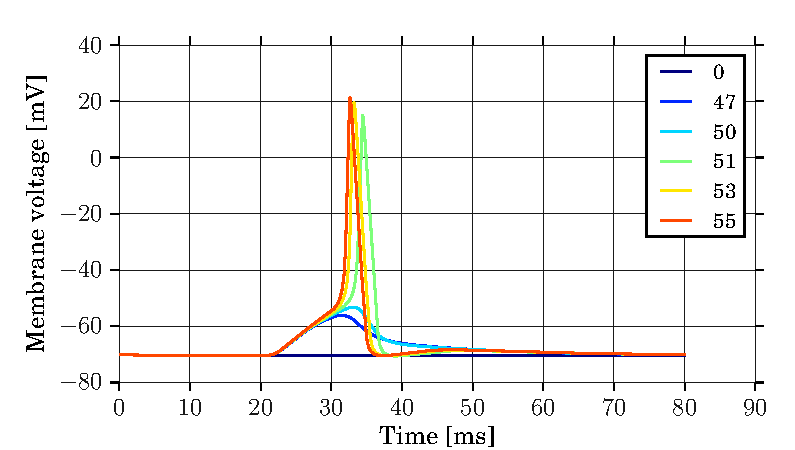
\includegraphics[width=\columnwidth]{../figures/2_1-dend2_synapse_number.pdf}
\end{center}
\label{fig:2_1_1}
\caption{Stimulus coming from dendrite 2 with different activated synapses}
\end{figure}

\begin{figure}
\begin{center}
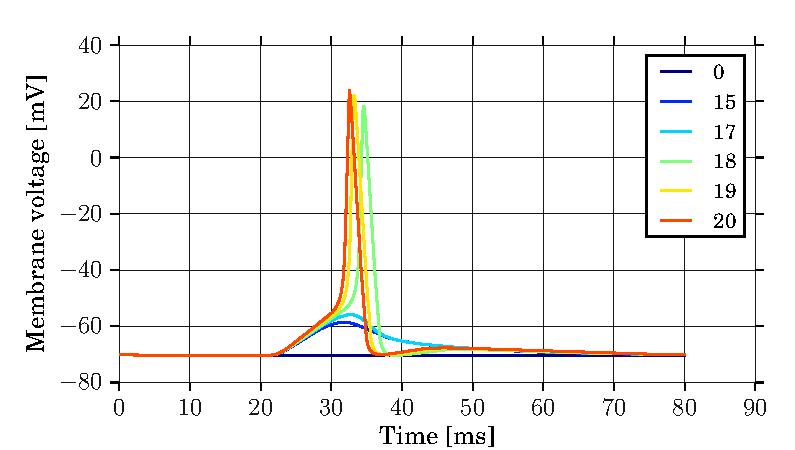
\includegraphics[width=\columnwidth]{../figures/2_1-dend3_synapse_number.pdf}
\end{center}
\label{fig:2_1_2}
\caption{Stimulus coming from dendrite 3 with different activated synapses}
\end{figure}

\begin{figure}
\begin{center}
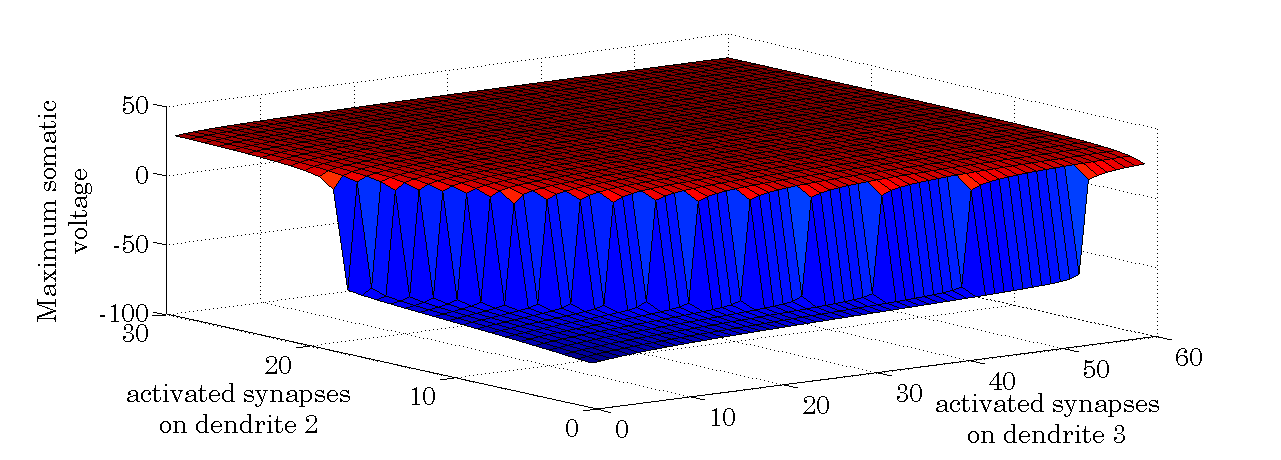
\includegraphics[width=\columnwidth]{../figures/2_2.png}
\end{center}
\label{fig:2_1_3}
\caption{Stimulus coming from dendrites 2 and 3 with different activated synapses for each dendrite}
\end{figure}

\subsection{Veto-inhibition} \label{sec:veto}
To make the synapse on dendrite 1 inhibitory, its conductance is set to a negative value. Its purpose is to “veto” an EPSP from the outer dendrites, by cancelling the spike. Two parameters are investigated for this: the onset time (relative to the synaptic onset) $\Delta t$, and maximum conductance g$_\text{max}$. \\

The inhibitory spike must reach its maximum at approximately the same time as the EPSP does, and its amplitude must be sufficient to cancel the EPSP spike. In order to find the values, a search on $\Delta t$ and g$_\text{max}$ was carried out. The optimal values to cancel a somatic spike created by opening 27 synapses on dendrite 3 were found to be $\Delta t$ = \SI{-5}{\milli\second} and g$_\text{max}$ = \SI{-0.0059}{\micro\siemens}. Since this synapse’s time constant is longer than the excitatory synapses (\SI{5}{\milli\second} vs \SI{2}{\milli\second}), it makes sense that it must be opened earlier. As for the value of the conductance, it is higher, simply because it has to compensate alone for the current from many other synapses. The fig. \ref{fig:2_1_4} shows the different maximum conductance for $\Delta t$ = \SI{-5}{\milli\second}.  \\

\begin{figure}
\begin{center}
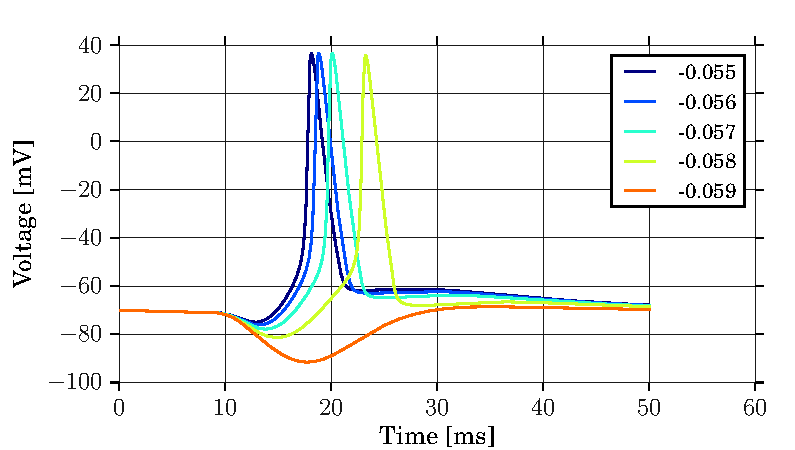
\includegraphics[width=\columnwidth]{../figures/2_3-veto_spike.pdf}
\end{center}
\label{fig:2_1_4}
\caption{Curve representing different value for g$_\text{max}$ value for $\Delta t$ equal to \SI{5}{\milli\second}.}
\end{figure}






\section{Conclusion}
Using simulations of Hodgkin-Huxley neurons, calculated by NEURON software, we observed the effects of non-linear ion channels on neuron behaviour, and the influence of dendritic properties on synaptic integration. First, knowing that the new ionic currents $I_x$ and $I_{xx}$ depend of the square of the voltage difference, they introduce non-linearity in the sub-threshold voltage in response to synaptic activation. For $I_x$ the relation becomes sub-linear and for $I_{xx}$ supra-linear, as determined by the sign of their respective maximal conductance.\\

Connecting dendrites with different characteristics influences the behaviours of the neuron. For example, a little stimulus on a dendrite 3 can generate a spike but the same stimulus on a dendrite 2 doesn't. Here again, the higher current leakage on dendrite 2 has the net effect of reducing its synaptic weight.\\

To inhibit a signal coming from an upstream dendrite, timing is critical, because the EPSP and IPSP should arrive at approximately the same time on the same location to cancel themselves. The maximal conductivity of the inhibitory synapse is important too, as it determines the amplitude of the IPSP.\\

\nocite{*}


\bibliographystyle{ieeetr}
\bibliography{neuron}

\end{document}
